\subsection{Understanding S Parameters: The Key to Input Port Reflection!}

\begin{tcolorbox}[colback=gray!10, colframe=black, title=E4B04] Which S parameter represents input port return loss or reflection coefficient (equivalent to VSWR)?

\begin{enumerate}[label=\Alph*.]
    \item \textbf{S11}
    \item S12
    \item S21
    \item S22
\end{enumerate} \end{tcolorbox}

\subsubsection*{Concepts Related to the Question}

In radio communication and electronics, S parameters, also known as scattering parameters, are essential for analyzing the behavior of electrical networks. Specifically, S parameters provide information about the reflection and transmission characteristics of a network when subjected to high-frequency signals.

The specific S parameters from the question include:
- \textbf{S11\textbf{: This parameter represents the input port reflection coefficient. It measures the ratio of the power reflected back from the input port when a signal is applied to it. A higher S11 value indicates less reflection and better matching, which corresponds to lower return loss or better Voltage Standing Wave Ratio (VSWR). Therefore, :}this is the correct answer}.
  
- S12: This parameter gives the transmission coefficient from port 1 to port 2, indicating how much power is transmitted through the network from the input side to the output side.

- S21: This parameter provides the transmission coefficient from port 2 to port 1, indicating how much power is transmitted through the network from the output side back to the input side.

- S22: Similar to S11, S22 represents the reflection coefficient at the output port, measuring how much power is reflected from the output.

\subsubsection*{Calculations and Examples}

To obtain the return loss (\( RL \)), which is related to S11, we can use the formula:

\[
RL = -20 \log_{10} |S_{11}|
\]

For example, if \( |S_{11}| = 0.1 \):
\[
RL = -20 \log_{10}(0.1) = -20 \times (-1) = 20 \, \text{dB}
\]

This indicates a return loss of 20 dB, meaning the input port has acceptable match characteristics.

\subsubsection*{Diagram Representation}

A simple schematic diagram can provide a better understanding of the concept. The following diagram uses TikZ to represent the input, output, and the S parameters.

\begin{center}
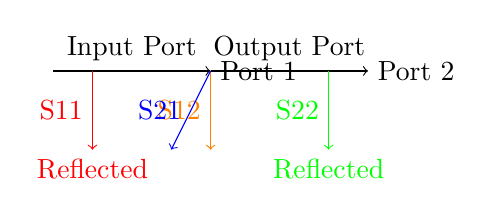
\begin{tikzpicture}
    \draw[->] (0,0) -- (2,0) node[midway, above] {Input Port} node[right] {Port 1};
    \draw[->] (2,0) -- (4,0) node[midway, above] {Output Port} node[right] {Port 2};
    \draw[->, red] (0.5,0) -- (0.5,-1) node[midway, left] {S11} node[below] {Reflected};
    \draw[->, green] (3.5,0) -- (3.5,-1) node[midway, left] {S22} node[below] {Reflected};
    \draw[->, orange] (2,0) -- (2,-1) node[midway, left] {S12};
    \draw[->, blue] (2,0) -- (1.5,-1) node[midway, left] {S21};
\end{tikzpicture}
\end{center}
